\documentclass[11pt,a4paper]{article}

% ─── Packages ────────────────────────────────────────────────────────────────
\usepackage[T1]{fontenc}
\usepackage{lmodern}
\usepackage[margin=2.5cm]{geometry}
\usepackage{amsmath,amssymb,amsthm}
\usepackage{mathtools}
\usepackage{graphicx}
\usepackage{bm}
\usepackage[pdftex,colorlinks=true,linkcolor=blue!60!black,
            citecolor=green!50!black,urlcolor=blue!60!black,
            pdfusetitle]{hyperref}
\usepackage{cleveref}
\usepackage{microtype}
\usepackage{enumitem}
\usepackage{booktabs}
\usepackage{array}
\usepackage{xcolor}
\usepackage{mdframed}
\usepackage[numbers,sort&compress]{natbib}
\usepackage{fancyhdr}
\pagestyle{fancy}
\fancyhf{}
\fancyhead[C]{\small\textit{Confidential draft --- not for sharing}}
\fancyfoot[C]{\thepage}
\renewcommand{\headrulewidth}{0.4pt}

% ─── Theorem environments ─────────────────────────────────────────────────────
\theoremstyle{definition}
\newtheorem{remark}{Remark}[section]
\newtheorem{definition}{Definition}[section]

\theoremstyle{plain}
\newtheorem{proposition}{Proposition}[section]

% ─── Custom commands ──────────────────────────────────────────────────────────
% Green's function and self-energy
\newcommand{\GG}{G}
\newcommand{\Sig}{\Sigma}
% Hubbard model
\newcommand{\tH}{t}
\newcommand{\UH}{U}
% Frequency arguments
\newcommand{\iw}{i\omega_n}
\newcommand{\wR}{\omega}
% Misc
\newcommand{\kB}{k_{\mathrm{B}}}
\newcommand{\half}{\tfrac{1}{2}}

% colour for highlight boxes
\definecolor{boxbg}{RGB}{240,246,255}
\definecolor{boxframe}{RGB}{70,130,180}

\newenvironment{keybox}[1]{%
  \begin{mdframed}[backgroundcolor=boxbg,linecolor=boxframe,linewidth=1pt,
    innertopmargin=6pt,innerbottommargin=6pt,innerrightmargin=8pt,innerleftmargin=8pt]
  \textbf{#1.}\quad}{\end{mdframed}}

% ─── Metadata ─────────────────────────────────────────────────────────────────
\title{\Large\bfseries Counterterm SOEHYB Run Instructions:\\
       Spinless and Spinful Hubbard Benchmarks\\[6pt]
       \normalsize\normalfont Reproducibility Notes}
\author{Emanuel Gull}
\date{\today}

% ═════════════════════════════════════════════════════════════════════════════

\begin{document}

\maketitle

\begin{abstract}
This note records the minimal commands and files needed to reproduce two
counterterm benchmarks of the semicircular-bath impurity problem with
\texttt{QMBToolkitSOEHYB.jl}.  The first is the easiest paper benchmark: a
non-interacting spinless impurity at $\beta t=8$ with three counterterms and a
bare hybridization expansion through $k=2$, compared directly to the analytic
semicircular-bath Green's function.  The second is an interacting spinful
Hubbard impurity at $\beta=8$, $U=2$, and half filling, used as a practical
scan over counterterm number $n_{\mathrm{CT}}$ and expansion order $k$.
\end{abstract}

\tableofcontents
\newpage

\section{Repository and Environment}

All commands are run from the \texttt{QMBToolkitSOEHYB.jl} package directory of a
checkout of \url{https://github.com/Green-Phys/green-jl-counterterms}:
\begin{verbatim}
git clone https://github.com/Green-Phys/green-jl-counterterms.git
cd green-jl-counterterms/QMBToolkitSOEHYB.jl
\end{verbatim}
Julia was installed with MacPorts and tested as
\begin{verbatim}
julia --version
# julia version 1.12.6
\end{verbatim}
The package tests passed for the local stack:
\begin{itemize}[leftmargin=*]
\item \texttt{QMBToolkitSOEHYB}: 214 tests passed.
\item \texttt{QMBToolkitED}: 440 tests passed.
\item \texttt{QMBToolkitDLR}: 8 tests passed.
\item \texttt{NumericsSOE}: 54 tests passed.
\end{itemize}

\begin{keybox}{Generator dependencies}
The light counterterm generator imports \texttt{ArgParse} and
\texttt{NumericsSOE}.  Add them to the \texttt{QMBToolkitSOEHYB.jl}
environment before running the generator:
\begin{verbatim}
cd green-jl-counterterms/QMBToolkitSOEHYB.jl
julia --project=. -e 'using Pkg; Pkg.add("ArgParse"); Pkg.develop(path="../NumericsSOE.jl"); Pkg.instantiate()'
\end{verbatim}
\end{keybox}

\section{Spinless Benchmark Parameters}

The paper benchmark is the non-interacting spinless Anderson impurity coupled
to a semicircular bath.  The bath density is
\begin{equation}
  \Gamma(\omega)=\frac{\sqrt{4t^2-\omega^2}}{2\pi t^2},
  \qquad -2t \leq \omega \leq 2t,
\end{equation}
with $t=1$ setting the energy unit.  The run documented here uses
\begin{align*}
  \beta t &= 8, & \beta &= 8,\\
  n_{\mathrm{CT}} &= 3, & k_{\max} &= 2.
\end{align*}
The physical impurity has zero onsite energy and no interaction.  The
counterterm construction enlarges the Hamiltonian by three auxiliary bath
levels, so the final \texttt{hopping.txt} is not zero even though the original
physical impurity is non-interacting.

\section{Generated Input Directory}

All files for this run are under
\begin{center}
\texttt{paper\_inputs/spinless\_beta8\_nct3\_k2/}
\end{center}
relative to the \texttt{QMBToolkitSOEHYB.jl} package directory.  The solver
input file is
\begin{center}
\texttt{paper\_inputs/spinless\_beta8\_nct3\_k2/input.toml}.
\end{center}
It points to the generated data files
\begin{verbatim}
data/hopping.txt
data/Uijkl.txt
data/hyb_poles.txt
data/hyb_weights.txt
\end{verbatim}
and writes the result to
\begin{verbatim}
output/sim.h5
\end{verbatim}

The solver-order convention is that the propagator expansion order counts
hybridization lines, while the Green's-function order is one larger.  Therefore
bare order $k=2$ is encoded as
\begin{verbatim}
[solver.propagator]
is_bold = false
expansion_order = 2

[solver.green]
is_bold = false
expansion_order = 3
save_linear_size = 1001
\end{verbatim}

\section{Commands}

Start from the package directory:
\begin{verbatim}
cd green-jl-counterterms/QMBToolkitSOEHYB.jl
\end{verbatim}

Create the paper-input directories:
\begin{verbatim}
mkdir -p paper_inputs/spinless_beta8_nct3_k2/data
mkdir -p paper_inputs/spinless_beta8_nct3_k2/output
\end{verbatim}

Generate the initial non-interacting spinless impurity Hamiltonian files:
\begin{verbatim}
julia --project=. scripts/gen_interaction_hopping.jl \
  --n_spin_impurity 1 \
  --n_orbital_impurity 1 \
  --t 0.0 \
  --U 0.0 \
  --J 0.0 \
  --Uprime 0.0 \
  --mu 0.0 \
  --output_dir paper_inputs/spinless_beta8_nct3_k2/data
\end{verbatim}
This creates \texttt{hopping.txt} and \texttt{Uijkl.txt}; before adding
counterterms, \texttt{Uijkl.txt} contains only \texttt{0}.

Fit the semicircular hybridization using the in-repository ESPRIT routine,
construct three counterterms, modify the hopping matrix, and write the residual
hybridization SOE:
\begin{verbatim}
julia --project=. scripts/gen_soe_counterterms_hyb_light.jl \
  --beta 8.0 \
  --n_spin_impurity 1 \
  --n_orbital_impurity 1 \
  --n_tau 1000 \
  --hyb_type SemiCircular \
  --hopping_file paper_inputs/spinless_beta8_nct3_k2/data/hopping.txt \
  --n_soe_counterterms 3 \
  --n_soe_hybridization 10 \
  --output_dir paper_inputs/spinless_beta8_nct3_k2/data \
  --do_subtraction_trick true
\end{verbatim}
The generator reported
\begin{verbatim}
Counterterm fit error = 2.410764606863666e-03
Residual SOE error    = 2.264410881025469e-12
Residual SOE poles    = 13
\end{verbatim}

Run the solver:
\begin{verbatim}
julia --project=. -e 'using QMBToolkitSOEHYB; QMBToolkitSOEHYB.run(ARGS[1])' \
  paper_inputs/spinless_beta8_nct3_k2/input.toml
\end{verbatim}
The run completed in about 35 seconds on one process and wrote
\texttt{output/sim.h5}.

\section{Output Check}

The HDF5 result contains the linear-grid Green's function at
\begin{verbatim}
/green/linear_grid/green_tau
/green/linear_grid/tau
\end{verbatim}
and the partition-function estimates at
\begin{verbatim}
/partition_function/partition_function_by_order
\end{verbatim}
For this run,
\begin{verbatim}
Z_by_order = [1.1272573397719343,
              1.127404158880327,
              1.1273824707953337]
\end{verbatim}
The first few computed Green's-function values were
\begin{verbatim}
tau = [0.0, 0.008, 0.016, 0.024]
G   = [-0.5000000000165467,
       -0.4966851837749550,
       -0.4934020226658121,
       -0.4901501755234226]
\end{verbatim}

\section{Comparison to Analytic Input}

The analytic/input curve was regenerated from the same semicircular bath used
by the generator, via \texttt{Lehmann.Sample.SemiCircle} on the DLR grid and
interpolated to the solver's linear grid.  The resulting comparison table is
\begin{center}
\texttt{paper\_inputs/spinless\_beta8\_nct3\_k2/output/green\_comparison.csv}.
\end{center}
The maximum absolute difference between the computed Green's function and the
input semicircular result is
\begin{equation}
  \max_\tau |G_{\mathrm{computed}}(\tau)-G_{\mathrm{input}}(\tau)|
  = 7.28\times 10^{-9}.
\end{equation}
The RMS difference is $3.61\times 10^{-9}$.

\begin{figure}[htbp]
  \centering
  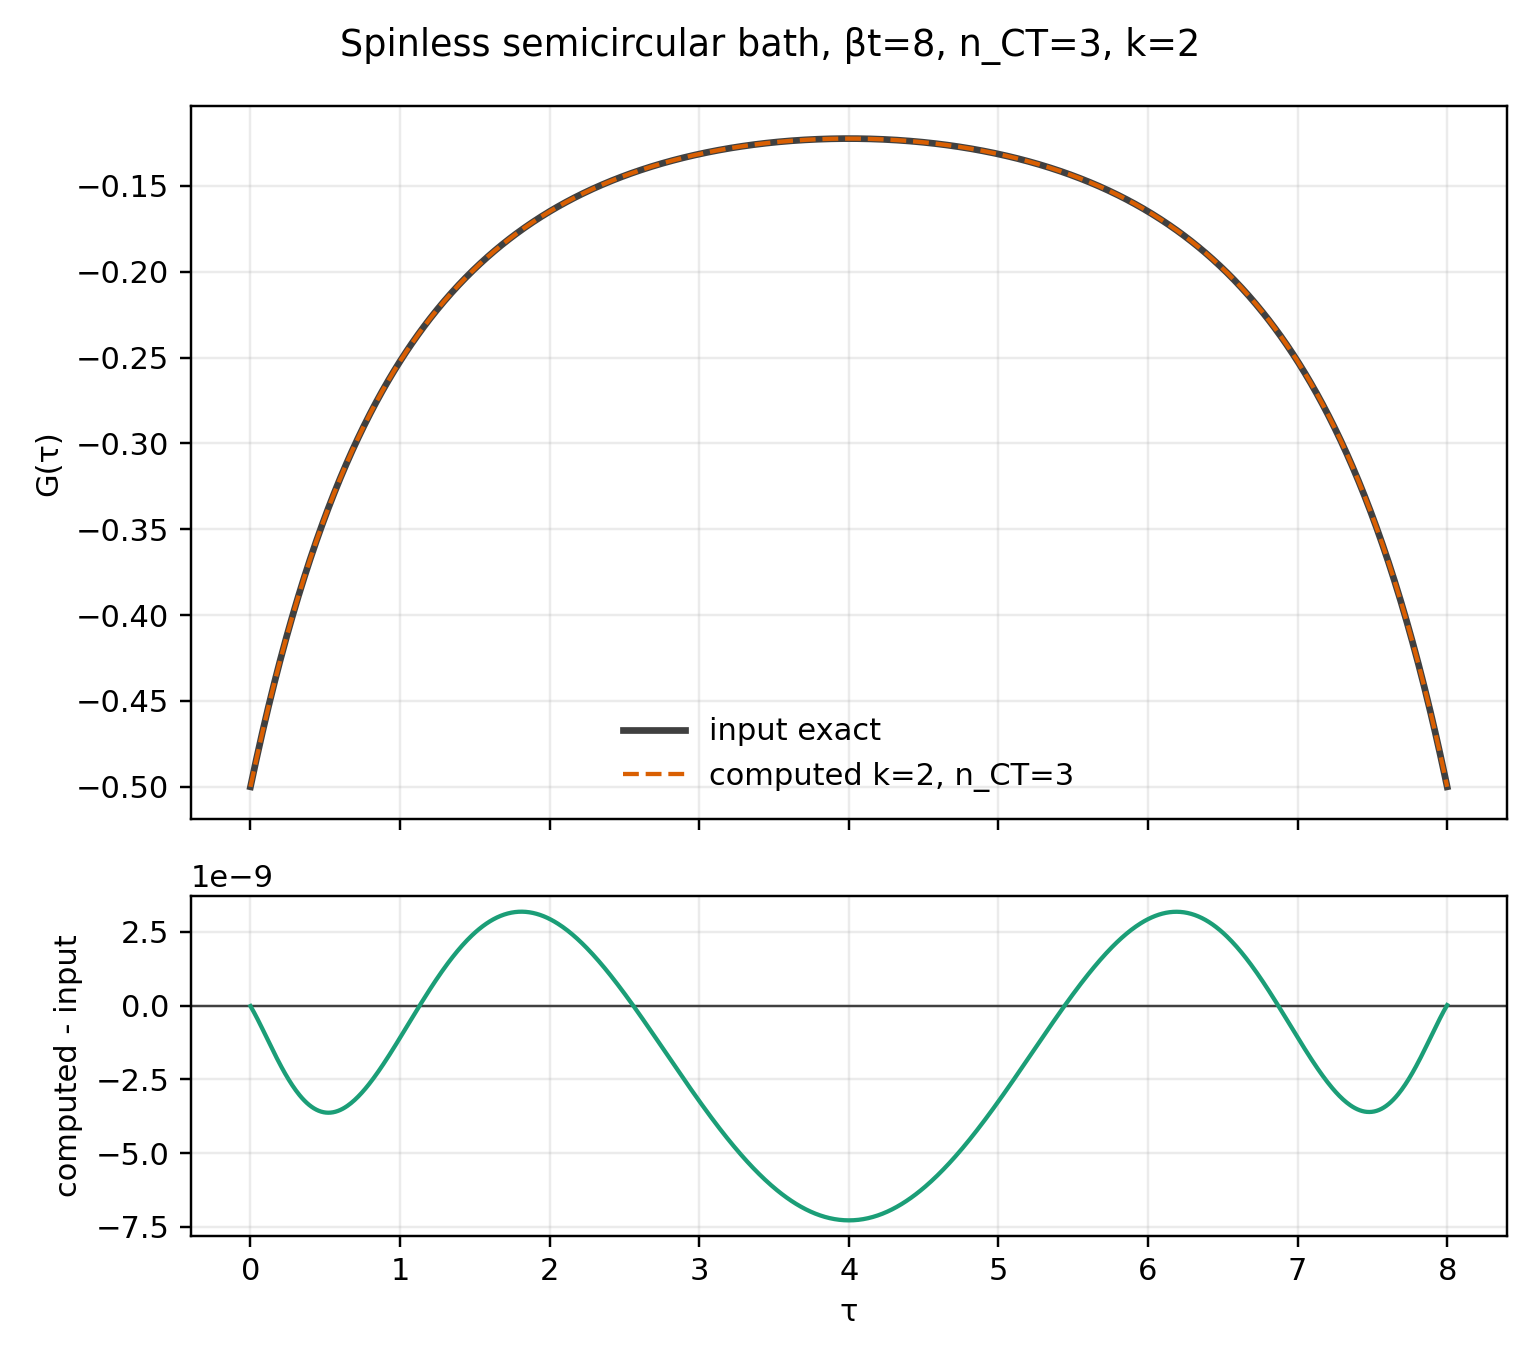
\includegraphics[width=0.95\linewidth]{figures/counterterm_green_comparison.png}
  \caption{Spinless semicircular-bath benchmark at $\beta t=8$ with
  $n_{\mathrm{CT}}=3$ and bare expansion through $k=2$.  Top: computed and
  analytic/input $G(\tau)$.  Bottom: computed minus input.}
  \label{fig:counterterm-green-comparison}
\end{figure}

\section{Interacting Spinful Hubbard Scan}

The simplest interacting case in this code path is the single-orbital spinful
Hubbard impurity coupled to the same semicircular bath.  The scan documented
here uses
\begin{align*}
  \beta &= 8, & U &= 2, & \mu &= U/2 = 1,\\
  n_{\mathrm{spin}} &= 2, & n_{\mathrm{orb}} &= 1, & t_{\mathrm{imp}} &= 0.
\end{align*}
The interaction file is therefore nonzero, unlike the spinless benchmark.  The
physical impurity has two flavors, spin up and spin down.  Counterterms add
auxiliary flavors, increasing the exact-diagonalization Hilbert space as
\begin{center}
\begin{tabular}{ccc}
\toprule
$n_{\mathrm{CT}}$ & total flavors & Fock-space dimension \\
\midrule
0 & 2 & 4 \\
1 & 4 & 16 \\
2 & 6 & 64 \\
3 & 8 & 256 \\
\bottomrule
\end{tabular}
\end{center}

The generated scan directory is
\begin{center}
\texttt{paper\_inputs/spinful\_hubbard\_beta8\_U2\_scan/}.
\end{center}
It contains one data directory per counterterm count and one solver input per
expansion order, for example
\begin{verbatim}
paper_inputs/spinful_hubbard_beta8_U2_scan/nct2/data/
paper_inputs/spinful_hubbard_beta8_U2_scan/nct2/k1/input.toml
\end{verbatim}
The helper script
\begin{center}
\texttt{paper\_inputs/spinful\_hubbard\_beta8\_U2\_scan/prepare\_inputs.py}
\end{center}
writes the \texttt{input.toml} files for $n_{\mathrm{CT}}=0,1,2,3$ and
$k=0,1,2$.  (This script is not yet part of the repository; each input has the
same form as the spinless \texttt{input.toml}, with \texttt{file\_path} pointing
to the \texttt{nct}$n$\texttt{/data} directory and the propagator and
Green's-function orders set to $k$ and $k+1$.)

\subsection{Generation Commands}

For each counterterm count, first generate the interacting impurity Hamiltonian:
\begin{verbatim}
julia --project=. scripts/gen_interaction_hopping.jl \
  --n_spin_impurity 2 \
  --n_orbital_impurity 1 \
  --t 0.0 \
  --U 2.0 \
  --J 0.0 \
  --Uprime 0.0 \
  --mu 1.0 \
  --output_dir paper_inputs/spinful_hubbard_beta8_U2_scan/nct${nct}/data
\end{verbatim}
Then fit the semicircular hybridization and build the counterterm Hamiltonian:
\begin{verbatim}
DATA=paper_inputs/spinful_hubbard_beta8_U2_scan/nct${nct}/data
julia --project=. scripts/gen_soe_counterterms_hyb_light.jl \
  --beta 8.0 \
  --n_spin_impurity 2 \
  --n_orbital_impurity 1 \
  --n_tau 1000 \
  --hyb_type SemiCircular \
  --hopping_file ${DATA}/hopping.txt \
  --n_soe_counterterms ${nct} \
  --n_soe_hybridization 10 \
  --output_dir ${DATA} \
  --do_subtraction_trick true
\end{verbatim}
The counterterm-fit errors decreased rapidly with $n_{\mathrm{CT}}$:
\begin{center}
\begin{tabular}{ccc}
\toprule
$n_{\mathrm{CT}}$ & counterterm fit error & residual SOE error \\
\midrule
0 & $5.0000\times 10^{-1}$ & $1.4250\times 10^{-12}$ \\
1 & $2.9345\times 10^{-1}$ & $1.4250\times 10^{-12}$ \\
2 & $2.9479\times 10^{-2}$ & $1.4250\times 10^{-12}$ \\
3 & $2.4108\times 10^{-3}$ & $1.4250\times 10^{-12}$ \\
\bottomrule
\end{tabular}
\end{center}

Run one case as
\begin{verbatim}
export INPUT=paper_inputs/spinful_hubbard_beta8_U2_scan/nct2/k1/input.toml
julia --project=. -e '
using QMBToolkitSOEHYB
QMBToolkitSOEHYB.run(ENV["INPUT"])
'
\end{verbatim}
The completed scan used all $n_{\mathrm{CT}}=0,1,2,3$ cases for $k=0,1$ and
$n_{\mathrm{CT}}=0,1,2$ for $k=2$.  The $n_{\mathrm{CT}}=3$, $k=2$ point was
left out because the $k=2$ cost already grew to several minutes by
$n_{\mathrm{CT}}=2$.

\subsection{Timing and Convergence}

The wall-clock timings below are from one MPI process.  The Green's-function
evaluation dominates the $k=2$ runs.
\begin{center}
\begin{tabular}{ccrrr}
\toprule
$n_{\mathrm{CT}}$ & $k$ & total (s) & propagator (s) & Green's function (s) \\
\midrule
0 & 0 & 3.15 & 2.11 & 0.88 \\
1 & 0 & 3.18 & 2.12 & 0.90 \\
2 & 0 & 3.20 & 2.12 & 0.92 \\
3 & 0 & 3.36 & 2.21 & 0.97 \\
0 & 1 & 3.52 & 2.36 & 1.00 \\
1 & 1 & 3.83 & 2.47 & 1.19 \\
2 & 1 & 4.61 & 2.65 & 1.79 \\
3 & 1 & 11.67 & 4.47 & 7.02 \\
0 & 2 & 24.42 & 6.19 & 18.07 \\
1 & 2 & 101.12 & 18.95 & 81.94 \\
2 & 2 & 412.99 & 70.47 & 342.31 \\
\bottomrule
\end{tabular}
\end{center}

The summary script
\begin{center}
\texttt{paper\_inputs/spinful\_hubbard\_beta8\_U2\_scan/summarize\_scan.py}
\end{center}
writes
\begin{verbatim}
spinful_hubbard_scan_summary.csv
spinful_hubbard_scan_summary.png
\end{verbatim}
Using the highest completed point, $n_{\mathrm{CT}}=2$, $k=2$, as an internal
reference, the closest completed point is $n_{\mathrm{CT}}=3$, $k=1$ with
\begin{equation}
  \max_\tau |G(\tau)-G_{\mathrm{ref}}(\tau)| = 5.97\times 10^{-5},
  \qquad
  \mathrm{RMS}=3.78\times 10^{-5}.
\end{equation}

\begin{figure}[htbp]
  \centering
  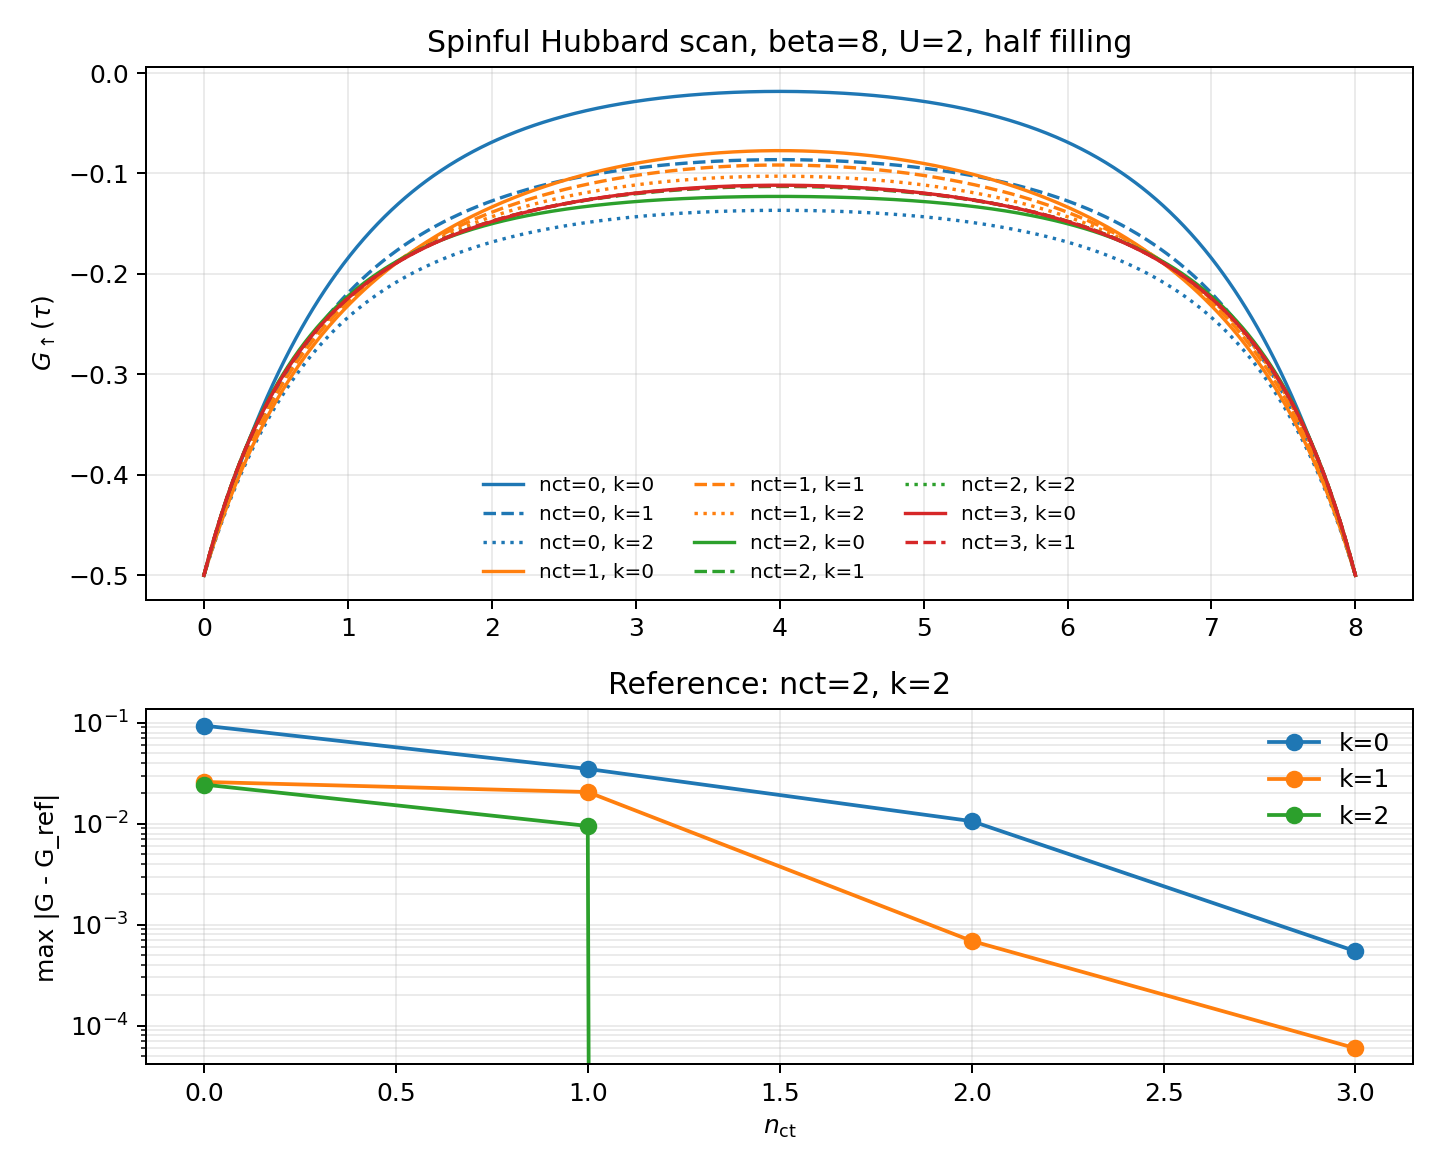
\includegraphics[width=0.95\linewidth]{figures/spinful_hubbard_scan_summary.png}
  \caption{Interacting spinful Hubbard scan at $\beta=8$, $U=2$, and half
  filling.  Top: $G_{\uparrow}(\tau)$ for completed $n_{\mathrm{CT}}$ and
  $k$ values.  Bottom: maximum difference from the $n_{\mathrm{CT}}=2$,
  $k=2$ internal reference.}
  \label{fig:spinful-hubbard-scan}
\end{figure}

\section{What Is Reproduced and What Is Not}

This note reproduces the easiest spinless case: the main-text setup at
$\beta t=8$, $n_{\mathrm{CT}}=3$, and $k=2$, and adds a practical interacting
spinful Hubbard scan at $\beta=8$, $U=2$, and half filling.  The spinful case
is an internal convergence check over $n_{\mathrm{CT}}$ and $k$; it is not an
external exact or CT-HYB benchmark.  The full paper figures also show broader
scans over $n_{\mathrm{CT}}$, expansion order, temperature, and comparisons to
external bold-line or CT-HYB data.  Those larger figure-generation datasets
were not present in the arXiv source bundle; they require additional benchmark
files or scripts.

\end{document}
